\documentclass[%
 reprint,
%superscriptaddress,
%groupedaddress,
%unsortedaddress,
%runinaddress,
%frontmatterverbose, 
%preprint,
%preprintnumbers,
%nofootinbib,
%nobibnotes,
%bibnotes,
 amsmath,amssymb,
 aps,
%href,
%colorlinks,
%pra,
%prb,
%rmp,
%prstab,
%prstper,
%floatfix,
]{revtex4-2}

\usepackage[T2A]{fontenc}
\usepackage[utf8x]{inputenc}
\usepackage{polyglossia}
\usepackage{tempora}
\setdefaultlanguage[indentfirst=true,forceheadingpunctuation=false]{russian}
\setotherlanguages{english}

\usepackage[toc]{glossaries}
\makeglossaries
\usepackage{graphicx}% Include figure files
\usepackage{dcolumn}% Align table columns on decimal point
\usepackage{bm}% bold math

\IfFontExistsTF{Times New Roman}
{\setmainfont{Times New Roman}
\newfontfamily\cyrillicfont{Times New Roman}[Script=Cyrillic]}
{\setmainfont[Script=Cyrillic]{FreeSerif}}

\IfFontExistsTF{Courier New}
{\setmonofont{Courier New}
\newfontfamily\cyrillicfonttt{Courier New}[Script=Cyrillic]}
{\setmonofont[Script=Cyrillic]{FreeMono}}

\IfFontExistsTF{Arial}
{\setsansfont{Arial}
\newfontfamily\cyrillicfontsf{Arial}[Script=Cyrillic]}
{\setsansfont[Script=Cyrillic]{FreeSans}}

%Доп пакеты для оформления
\usepackage{graphicx}% Include figure files
\usepackage{dcolumn}% Align table columns on decimal point
\usepackage{bm}% bold math
\usepackage{icomma} %Интеллектуальная запятая в десятичной записи числа
%\usepackage{longtable}

% Начало документа

\begin{document}

\preprint{APS/123-QED}

\title{
    Атомистическое и континуальное моделирование \\
    адиабатического расширения вещества с потенциалом Леннарда-Джонса
}% Force line breaks with \\

\author{Левашов Павел Ремирович}
\affiliation{
 Объединённый институт высоких температур РАН
}%

\author{Фолифоров Даниил Сергеевич}
\affiliation{%
 Московский физико-технический институт\\
 foliforov.ds@phystech.edu
}%

\date{\today}% It is always \today, today,
             %  but any date may be explicitly specified

\begin{abstract}
An article usually includes an abstract, a concise summary of the work
covered at length in the main body of the article. 
\begin{description}
\item[Usage]
Secondary publications and information retrieval purposes.
\item[Structure]
You may use the \texttt{description} environment to structure your abstract;
use the optional argument of the \verb+\item+ command to give the category of each item. 
\end{description}
\end{abstract}

%\keywords{Suggested keywords}%Use show keys class option if keyword
                              %display desired

\maketitle

% Раздел 1: Введение
\section{\label{sec:level1}First-level heading}

sample document

% Раздел 2: Методика эксперимента
\section{\label{sec 2}Методика эксперимента}

В данной работе для формирования изоэнтропы разгрузки металла была смоделирована задача о распаде произвольного разрыва. Для этого сжатый металл расширялся в область с меньшим значением плотности системы. В этих условиях, основываясь на гидродинамическом анализе, ударная волна сжатия распространяется в преграду, а в металл – волна разрежения.

В этой работе для анализа термодинамических свойств веществ на атомарном уровне было выполнено 
молекулярно-динамическое моделирование распада произвольного разрыва между исследуемым металлом и преградой. Все расчеты осуществлялись с использованием открытого программного пакета для решения задач молекулярной динамики LAMMPS. Термостатирование моделируемых систем проводилось с применением алгоритма Нозе–Гувера.

Проведение эксперимента по изоэнтропическому расширению в двухфазную область предусматривает разделения моделирования
на два ключевых этапа: подготовка сжатого образца, состоящего из атомов единственного вещества, и преград различной 
плотности; непосредственное моделирование изоэнтропичсекого расширения. В экспериментальных исследованиях получение 
сжатого образца является важным этапом работы, который на практике осуществляется, зачастую, при помощи ударно-взрывного воздействия. Схожий процесс возможно реализовать и в программном пакете LAMMPS с использованием алгоритма, предложенного Оскаром Герреро-Мирамонтесом. Однако в данной работе рассматривается идеализированная постановка задачи, в рамках которой исследуемый образец уже находится в сжатом состоянии с известными термодинамическими значениями. Описанное упрощение позволяет сократить время проведения серий экспериментов и не усложняет процесс подбора начальных условий.

В качестве межчастичного потенциала взаимодействия в данной работе использовался потенциал \acrfull{lj}. Данный потенциал является наиболее широко используемым потенциалом межмолекулярного взаимодействия в истории моделирования, который достаточно хорошо описывает поведение небольших сферических и неполярных молекул. Он был широко изучен в последние десятилетия и может служить реалистичной моделью для изучения фазовых равновесий, процессов фазового перехода, поведения кластеризации или свойств переноса простых жидкостей.

Наиболее часто встречающееся в литературе выражение для данного потенциала записывается следующим образом:
\begin{equation}
    U_{LJ} = 4\varepsilon\left[\left(\frac{\sigma}{r}\right)^{12} - \left(\frac{\sigma}{r}\right)^{6}\right],
    \label{eq:LJ}
\end{equation}
%
где $r$$~-$ расстояние между двумя взаимодействующими частицами, $\varepsilon$$~-$ энергетическая константа (или глубина потенциальной ямы), а $\sigma$$~-$ расстояние, на котором потенциальная энергия межчастичного взаимодействия равна нулю (часто называемая «размер частицы»). Параметры $\varepsilon$ и $\sigma$, определяемые подгонкой к известным свойствам вещества, соответствуют энергии и длине связи соответственно, измеряются экспериментально и являются его характеристиками.

В качестве вещества, находящегося в сжатом состоянии, был взят металл молибден (Mo). Данный выбор был обусловлен наличием экспериментальных, которые необходимо было проанализировать на атомарном уровне для уточнения процессов, происходящих при его попадании в двухфазную область.
% Необходимо внести параметры потенциала ЛД.  
В качестве преграды использовался аргон (Ar). Атомы данного инертного газа является достаточно лёгкими, что позволяет применять его для моделирования преград различной плотности в широком диапазоне значений, включающих предельно малые плотности.
% Необходимо внести параметры потенциала ЛД. 

Процесс моделирования начинался с выбора значений плотности ($\rho$) и температуры ($T$) на фазовой диаграмме с низкими значениями давлений ($P$). Методика эксперимента позволяет сделать это упрощение, ускоряя процесс расчётов и упрощая подбор параметров ячейки симуляции. 

Сама окно моделирования представляет собой прямоугольник значительно вытянутый по одной из осей в длину, на который наложены периодические граничные условия. При задании начальных параметров образца атомы вещества располагаются в узлах ГЦК-решётки, а в случае симуляции преград их распределение определяется произвольным образом. После чего начинается процесс моделирования в NVE-ансамбле с использование термостата. Результатом которого является приведение вещества в состояние термодинамического равновесия с заданными и известными значениями плотности и температуры.

На следующем этапе моделирования распада произвольного разрыва боковые грани подготовленных образца и преграды приводились в соприкосновение (для ясности будем называть оси соприкосновения $Ox$ и $Oy$). Полученная таким образом прямоугольная ячейка представляет вытянутый вдоль одной оси ($Oz$) прямоугольный параллелепипед. Используемая конфигурация позволяет на протяжении достаточного промежутка времени фиксировать распространение ударной и разгрузочной волн вдоль $Oz$. При этом важно отметить, что такая постановка эксперимента накладывают ограничение на использование периодических граничных условий по $Oz$ для предотвращения воздействия мнимых частиц преграды на образец. В связи с этим, для предотвращения разлёта частиц, по краям ячейки моделирования располагаются отражающие "зеркальные" границы. Компонента вектора скорости $z$ движущегося атома, при соприкосновении с ними, меняется на противоположную, при этом модуль вектора скорости сохраняется. Важно отметить, что переодические граничные условия по осям $Ox$ и $Oy$ сохраняются.

Дальнейший процесс моделирования распада произвольного разрыва проводился в микроканоническом ансамбле $NVE$. Для наблюдения за распространением волн ячейка симуляции делилась на тонкие продольные срезы по оси $Oz$. В каждом из которых рассчитывались усреднённые термодинамические величины через равные промежутки времени.  

% Раздел 3: Тестовый расчёт изоэнтропы разгрузки
\section{\label{sec 3}Тестовый расчёт изоэнтропы разгрузки}

В качестве исходной точки на фазовой диаграмме было вобрано такое состояние $Mo$, находящегося в области высокого давления, для которого изоэнтропа разгрузки однозначно пересекает бинодаль и попадает в двухфазную область жидкость-газ. Для того, чтобы убедиться в корректности выбора начального положения, в данной работе были использованы уравнение состояния вещества с потенциалом \acrshort{lj}, полученные в \cite{Ahmed:JCP:2009, Heier:MP:2018,Watanabe:JCP:2012, Adidharma:JCP:2016, THOL:JPCRF:2016}. Для тестового расчёта была выбрана термодинамическая система, удовлетворяющая описанным условия,  со следующими характеристиками: $T_{sample, t=0} = 5$ и $\rho_{sample, t=0} = 1.25$. Из предложенной точки на фазовой диаграмме была построена изоэнтропа Рис.\ref{fig:iso_S}.    

\begin{figure}[ht]
    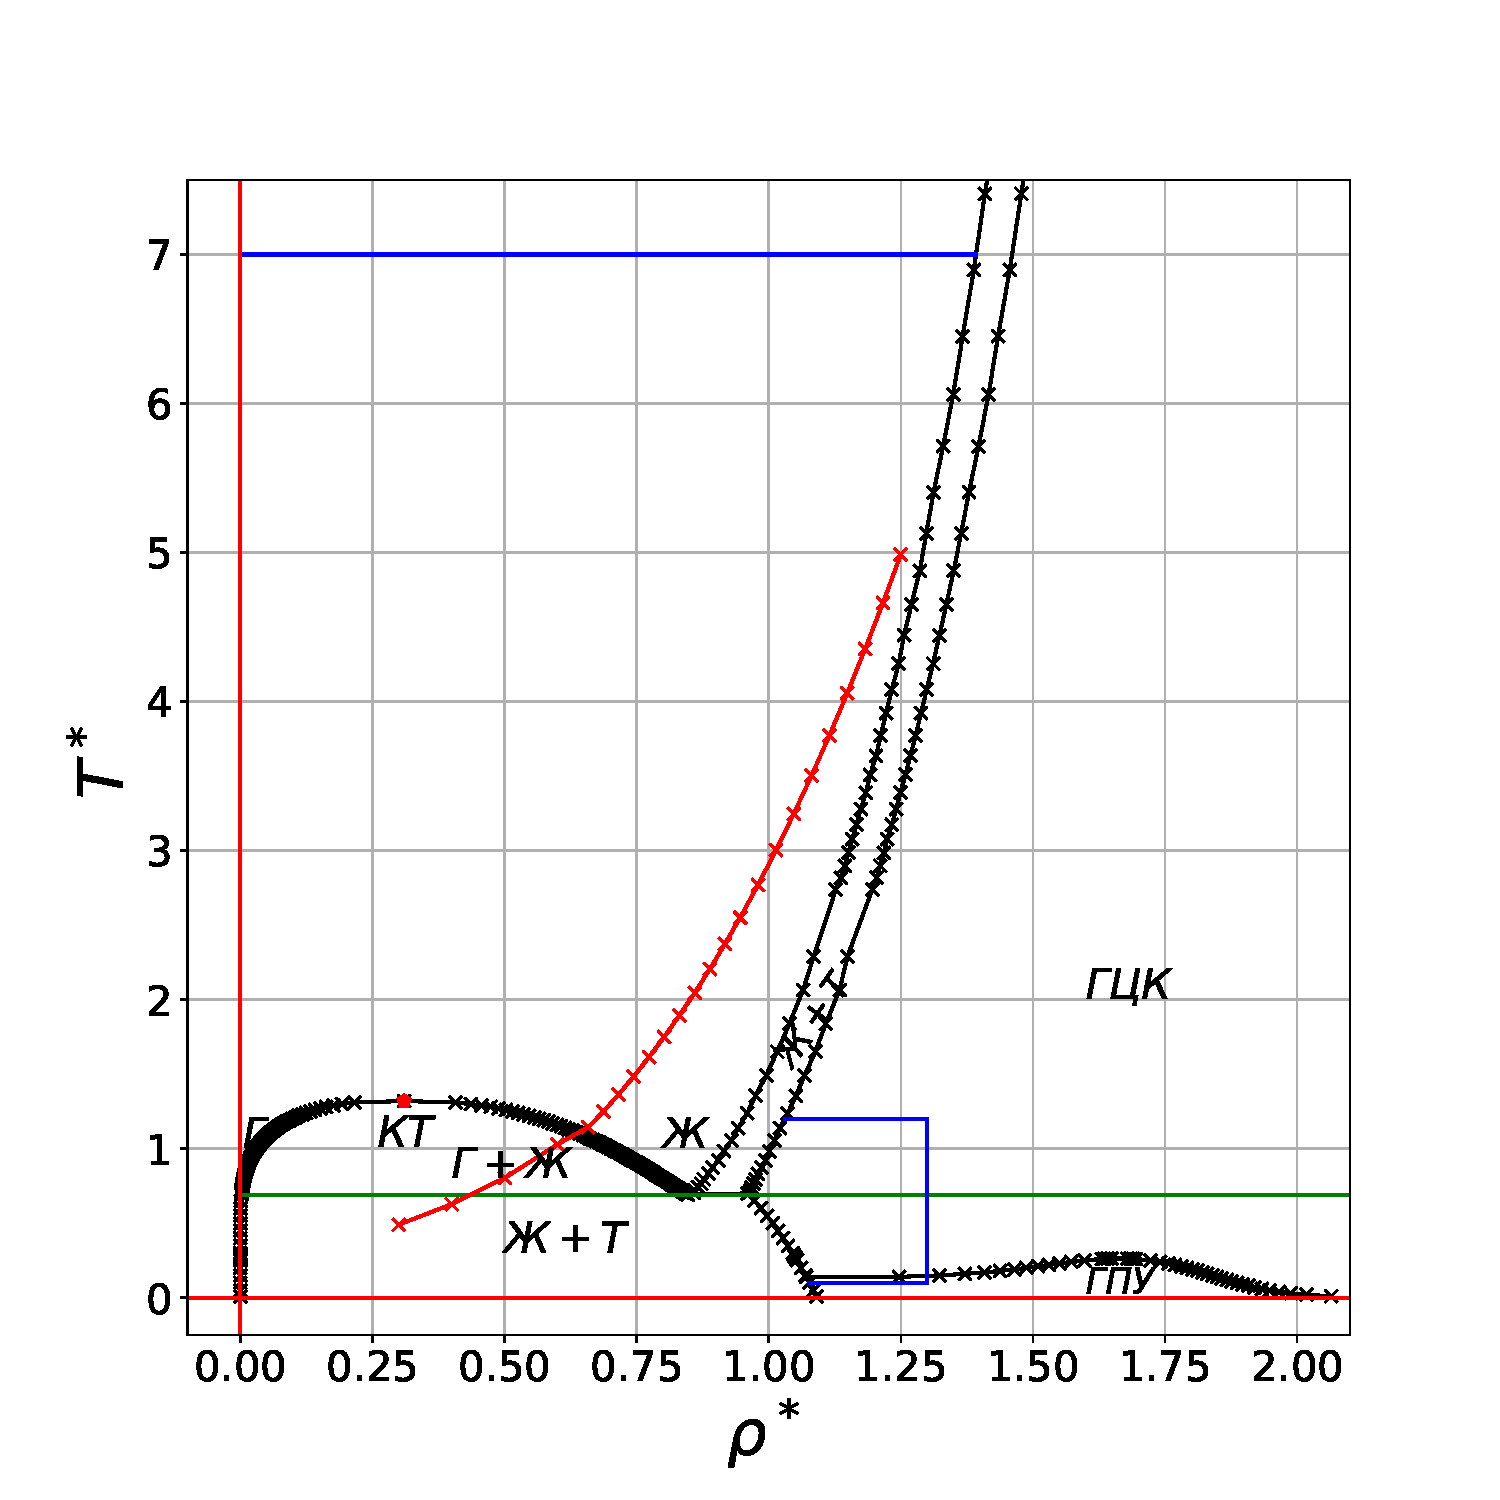
\includegraphics[width=\linewidth]{img/Isontropa.pdf}
    \caption{\label{fig:iso_S} График изоэнтропы на фазовой диаграмме. Основные фазовые состояния вещества: $Г$ $~-$ пар, $Ж$ $~-$ жидкость, \textit{ГЦК/ГПУ} $~-$ кристаллическое состояние вещества с двумя типами решеток (\acrshort{fcc} и \acrshort{hcp}, соответственно). Область \textit{Ж+Т} соответствует области плавления вещества, \textit{Ж+Г}$~-$ области сублимации и \textit{Г+Ж} $~-$ области испарения. Красной точкой \textit{КТ} на графике показана критическая точка, значения плотности и давления в ней равны, соответственно, $\rho_c = 0.31$ и $T_c = 1.32$. Зелёная прямая, проведённая параллельно оси $\rho^*$, показывает значение температуры в тройной точке на фазовой диаграмме, численно равное $T_{triple} = 0.692$. Плотности различных фаз в тройной точке равны, соответственно, $\rho_V = 0.0018$, $\rho_L = 0.847$, $\rho_S = 0.962$ \cite{Baidakov:JETP:2006}. Области на графике, образованные синими прямыми и чёрными кривыми фазовых состояний, показывают границы применимости уравнений состояний для соответствующих фаз.}
\end{figure}

При работе с потенциалом \acrshort{lj} удобно выражать термодинамические величины, такие как температура, плотность, давление и т.д., в безразмерных единицах измерения. Это означает, что необходимо выбрать удобную единицу измерения энергии, длины и массы, а затем получить все другие величины в пересчете на эти базовые единицы измерения. Исходя из записи \acrshort{lj}, естественно за основные принять следующие параметры: $\sigma$ $~-$ единица длины, $\varepsilon$ $~-$ единица энергии, $m$ $~-$ единица массы (масса атомов, участвующих в моделировании). И из этих базовых единиц измерения вытекают все остальные:

\begin{table}[h]
    \caption{\label{tab:table1} Приведённые термодинамические величины \acrshort{lj}}
    \begin{ruledtabular}
        \begin{tabular}{ l l l l }
            Расстояние & $r^* = r/\sigma$ & Энергия & $E^* = E/\varepsilon$\\
            Время & $t^* = t[\varepsilon/(m\sigma^2)]^\frac{1}{2}$ & Температура & $T^* = k_BT/\varepsilon$\\
            Масса & $m^* = m$ & Плотность & $\rho^* = \rho\sigma^3/m$\\
            Сила & $F^* = F\sigma/\varepsilon$ & & \\
        \end{tabular}
    \end{ruledtabular}
\end{table}

Затем из полученного графика было найдено значение плотности в месте пересечения построенной кривой с бинодалью, которое равняется $\rho_{binodal}=0.645$ единицам. Важно отметить данный факт, т.к. в дальнейшем значения плотности вещества за волной разгрузки будут сравниваться с $\rho_{binodal}$, что позволит определить в какой области фазовой диаграммы находится образец: флюидной или двухфазной \textit{Ж+Г}.  

% Раздел 4: Моделирование распада произвольного разрыва
\section{\label{sec 4}Моделирование распада произвольного разрыва}

\subsubsection{Вход в двухфазную область жидкость-газ}

Было проведено МД-моделирование входа изоэнтропы разгрузки алюминия в двухфазную область жидкость–газ. Начальные характеристики исследуемого металла $Mo$ были следующими: $T_{sample, t=0} = 5$ и $\rho_{sample, t=0} = 1.25$; а соответствующие характеристики барьера из атомов $Ar$: $T_{barrier, t=0} = 0.7$ и $\rho_{barrier, t=0} = 0.001$.

\begin{figure*}[ht]
    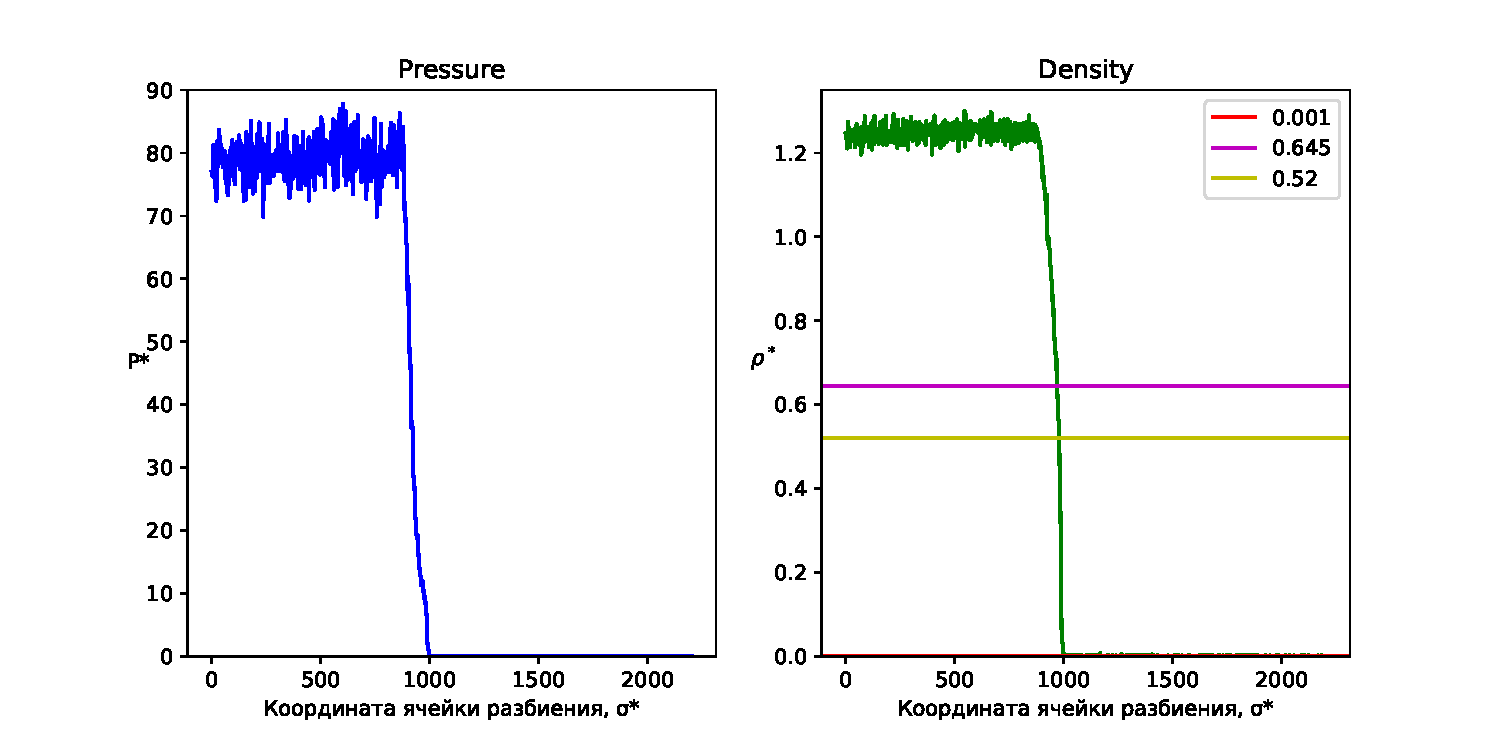
\includegraphics[width=\linewidth]{img/example_0.001/relax_wave3850.pdf}
    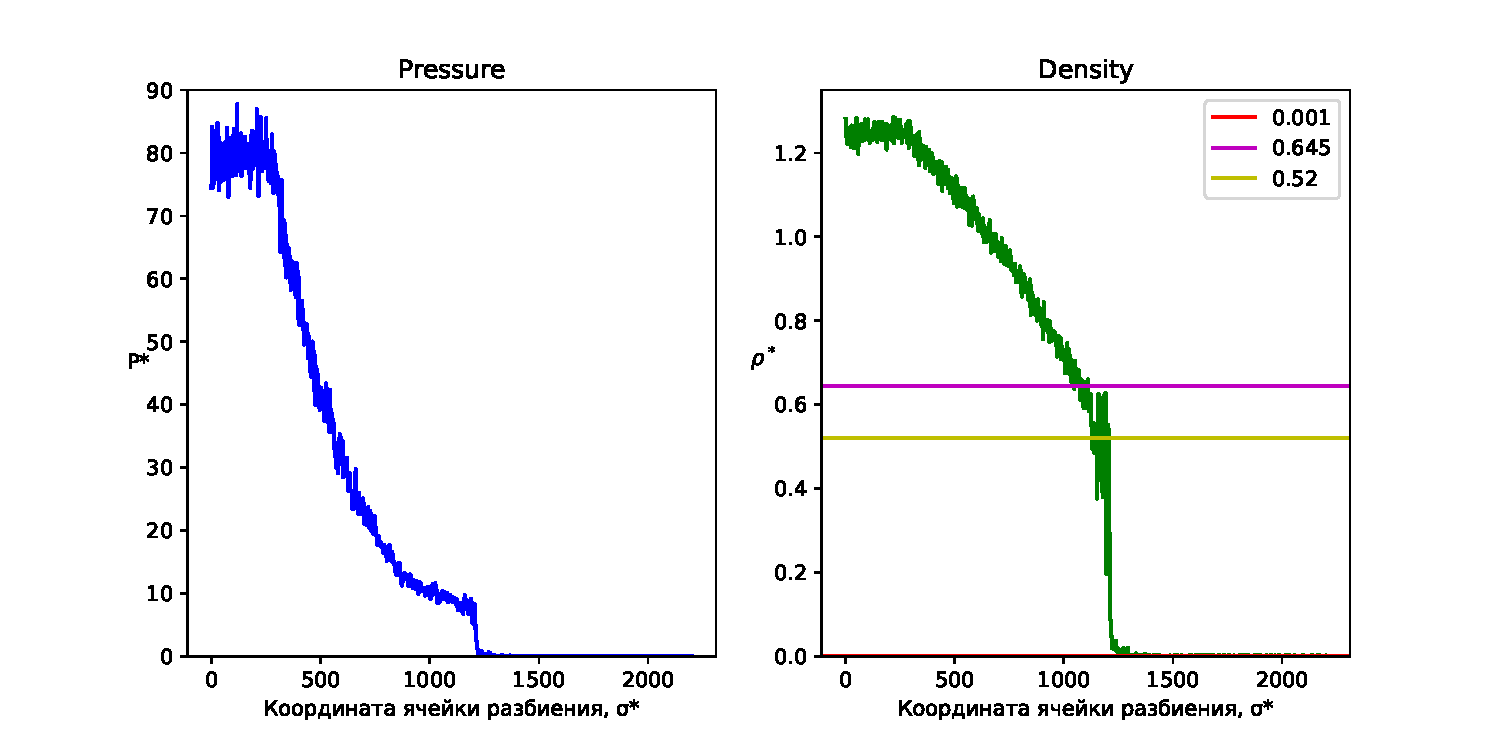
\includegraphics[width=\linewidth]{img/example_0.001/relax_wave36650.pdf}
    \caption{\label{fig:s_0.001} Моделирование в режиме ударной трубы, профили давления и плотности: верхний на шаге 3850, нижний на шаге 36650. Две горизонтальные линии на графике плотности обозначают, обсужденное ранее, значение плотности в точки пересечения изоэнтропы с бинодалью и значение плотности в образце, после прохождения по нему волны разрежения.}
\end{figure*}

Профили давления и плотности, полученные на разных этапах моделирования, представлены на рисунке \ref{fig:s_0.001}. Рассмотрим более детально полученные графики, в результате распада произвольного разрыва в области образца $Reg_{sample}$, состоящей из атомов $Mo$, и в области преграды $Reg_{barrier}$, состоящей из атомов $Ar$. В $Reg_{sample}$ наблюдаются плавные изменения распределения параметров $𝑃$ и $\rho$ относительно начальных значений, причем профили соответствуют движению волны разрежения влево от поверхности разрыва. В $Reg_{barrier}$, напротив, наблюдаются скачкообразные изменения этих параметров, что свидетельствует движению ударной волны сжатия вправо от поверхности разрыва. Значение плотности образца за волной разряжения, в приведённом эксперименте, соответственно равняется $0.52$. Полученная величина является меньшей по сравнению со значением плотности $0.645$ в точке пересечения изоэнтропы с бинодалью, что свидетельствует о проникновении внутрь двухфазной области жидкость-газ.

\begin{figure*}[ht]
    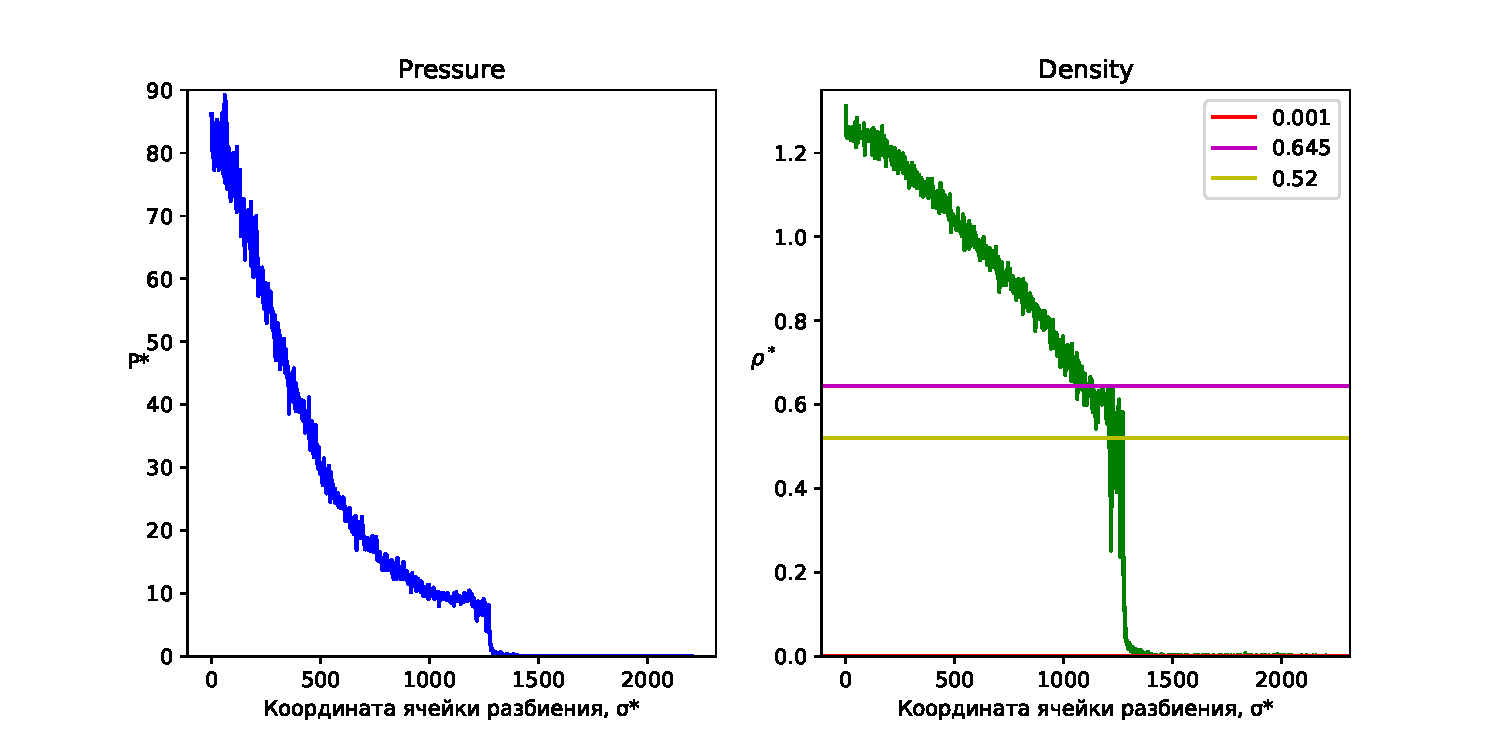
\includegraphics[width=\linewidth]{img/example_0.001/relax_wave46650.pdf}
    \caption{\label{fig:s_0.001_46650} Моделирование в режиме ударной трубы, профили давления и плотности на шаге 46650. Две горизонтальные линии на графике плотности обозначают, обсужденное ранее, значение плотности в точки пересечения изоэнтропы с бинодалью и значение плотности в образце, после прохождения по нему волны разрежения.}
\end{figure*}

Однако дальнейшее моделирование (рис. \ref{fig:s_0.001_46650}) показывает, что однородное состояние не успевает сформироваться. На графике плотности наблюдаются сильные флуктуации внутри двухфазной области. Однородное состояние быстро разрушается, и система стремится вернуться в более стабильную однофазную область. 

\subsubsection{Исследование волнового течения на границе двухфазной области}

С целью выяснения причины расхождения теоретического гидродинамического решения задачи распада произвольного разрыва и непосредственных результатов проведённого эксперимента была проведена серия моделирований с использованием преград различной плотности, чтобы проанализировать эффекты возникающие внутри двухфазной области, препятствующие образованию однородного состояния. 

\begin{figure}[ht]
    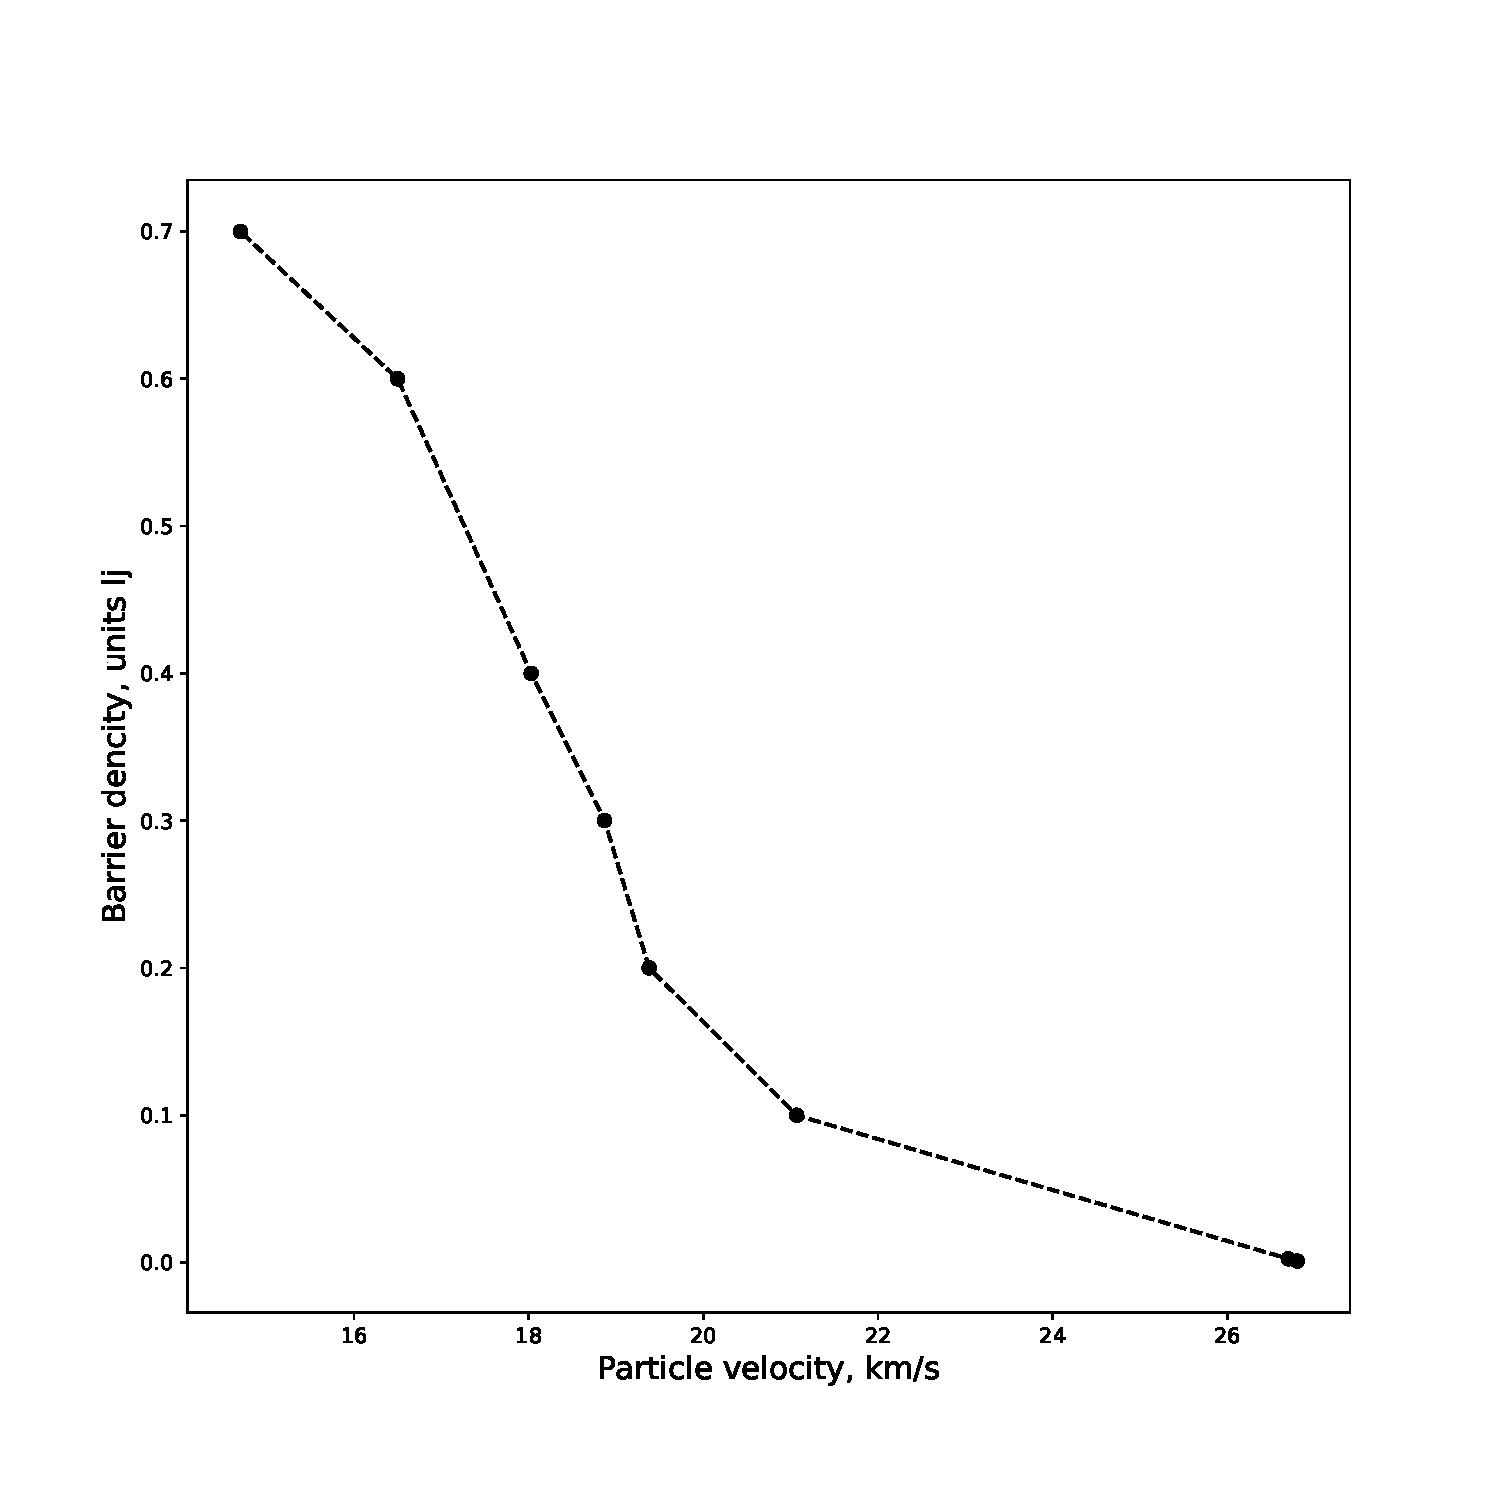
\includegraphics[width=\linewidth]{img/speed_comp.pdf}
    \caption{\label{fig:speed} График зависимости скорости распространения ударной волны в преграде.}
\end{figure}

На приведённом рисунке \ref{fig:speed} заметен характерный излом на изоэнтропе разгрузки, при использовании преград малой плотности. Как было показано ранее, данные значения плотности, позволяют веществу после разгрузки попасть внутрь двухфазной области. Однако изменение скорости распространения вещества перед фронтом ударной волны, указывает на образование быстрый излёт частиц вглубь невозмущённого вещества, приводящий к образованию струевидных течений. 

% Список сокращений
\newacronym{lj}{ЛД}{Леннарда-Джонса}
\newacronym{fcc}{ГЦК}{Гранецентрированная кубическая}
\newacronym{hcp}{ГПУ}{Гексагональная плотноупакованная}

\printglossaries
\bibliographystyle{unsrtnat}
\bibliography{simpl}
%\printbibliography[heading=bibintoc]
%\bibliographystyle{aspb1}
%\addbibresource{thesis.bib}
%\addbibresource{thesis}

\end{document}